\documentclass[tikz,border=3pt]{standalone}
\usepackage[utf8]{inputenc}
\usepackage[T1]{fontenc}
\usepackage{lmodern}
\renewcommand{\familydefault}{\sfdefault}
\usepackage{sansmath}\sansmath
\usepackage{chemfig}
\usepackage{pgfplots}\pgfplotsset{compat=1.18,/pgf/number format/use comma,/pgf/number format/1000 sep={.}}
\usetikzlibrary{arrows.meta,calc,positioning,decorations.pathmorphing,patterns}
% paleta del sitio
\definecolor{nar}{HTML}{E8680C}\definecolor{narc}{HTML}{FFB35C}\definecolor{hielo}{HTML}{FFF3E8}
\definecolor{tinta}{HTML}{1D1D1F}\definecolor{gris}{HTML}{6E6E73}\definecolor{lila}{HTML}{7C5CF0}
\definecolor{azul}{HTML}{2F6FD6}\definecolor{menta}{HTML}{17A673}\definecolor{coral}{HTML}{E8342A}
\begin{document}
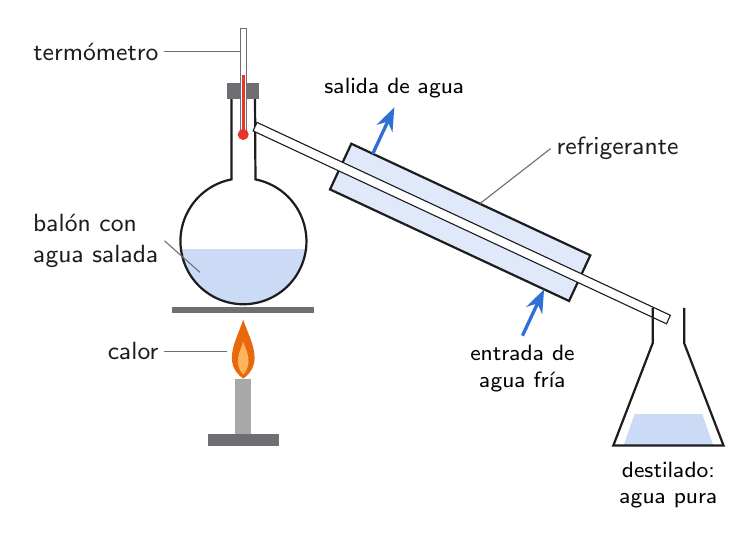
\begin{tikzpicture}[font=\small]

\fill[gris] (-0.45,0) rectangle (0.45,0.15);
\fill[gris!60] (-0.1,0.15) rectangle (0.1,0.85);
\fill[nar] (0,0.85) .. controls (-0.28,1.05) and (-0.08,1.35) .. (0,1.6) .. controls (0.08,1.35) and (0.28,1.05) .. (0,0.85);
\fill[narc] (0,0.9) .. controls (-0.13,1.05) and (-0.04,1.2) .. (0,1.32) .. controls (0.04,1.2) and (0.13,1.05) .. (0,0.9);
\draw[gris,line width=2pt] (-0.9,1.72) -- (0.9,1.72);
\begin{scope}\clip (0,2.6) circle (0.8); \fill[azul!25] (-1,1.7) rectangle (1,2.5); \end{scope}
\fill[white] (-0.15,3.3) rectangle (0.15,4.4);
\draw[tinta,thick] (-0.15,4.4) -- (-0.15,3.38) arc (101:439:0.8) -- (0.15,4.4);
\fill[white] (0,2.6) circle (0.02);
\draw[tinta,thick,fill=azul!15] (1.373,3.833) -- (4.408,2.416) -- (4.138,1.836) -- (1.102,3.253) -- cycle;
\draw[tinta,fill=white] (0.175,4.104) -- (5.425,1.654) -- (5.375,1.546) -- (0.125,3.996) -- cycle;
\draw[azul,very thick,-{Stealth}] (3.546,1.395) -- (3.821,1.984);
\node[anchor=north,align=center,font=\footnotesize] at (3.546,1.395) {entrada de\\agua fría};
\draw[azul,very thick,-{Stealth}] (1.645,3.706) -- (1.919,4.295);
\node[anchor=south,font=\footnotesize] at (1.919,4.295) {salida de agua};
\draw[gris] (3.004,3.071) -- (3.904,3.771) node[anchor=west,text=tinta,align=left,inner sep=2pt] {refrigerante};

\fill[gris] (-0.2,4.4) rectangle (0.2,4.6);
\draw[gris,fill=white] (-0.04,3.95) rectangle (0.04,5.3);
\fill[coral] (0,3.95) circle (0.07);
\fill[coral] (-0.02,3.95) rectangle (0.02,4.7);
% erlenmeyer
\fill[azul!25] (4.83,0) -- (5.97,0) -- (5.83,0.4) -- (4.97,0.4) -- cycle;
\draw[tinta,thick] (5.2,1.75) -- (5.2,1.3) -- (4.7,0) -- (6.1,0) -- (5.6,1.3) -- (5.6,1.75);
\draw[gris] (-0.04,5) -- (-1,5) node[anchor=east,text=tinta,align=left,inner sep=2pt] {termómetro};
\draw[gris] (-0.55,2.2) -- (-1,2.6) node[anchor=east,text=tinta,align=left,inner sep=2pt] {balón con\\agua salada};
\draw[gris] (-0.2,1.2) -- (-1,1.2) node[anchor=east,text=tinta,align=left,inner sep=2pt] {calor};
\node[anchor=north,align=center,font=\footnotesize] at (5.4,-0.08) {destilado:\\agua pura};

\end{tikzpicture}
\end{document}
